\begin{figure}[h]
    \centering
    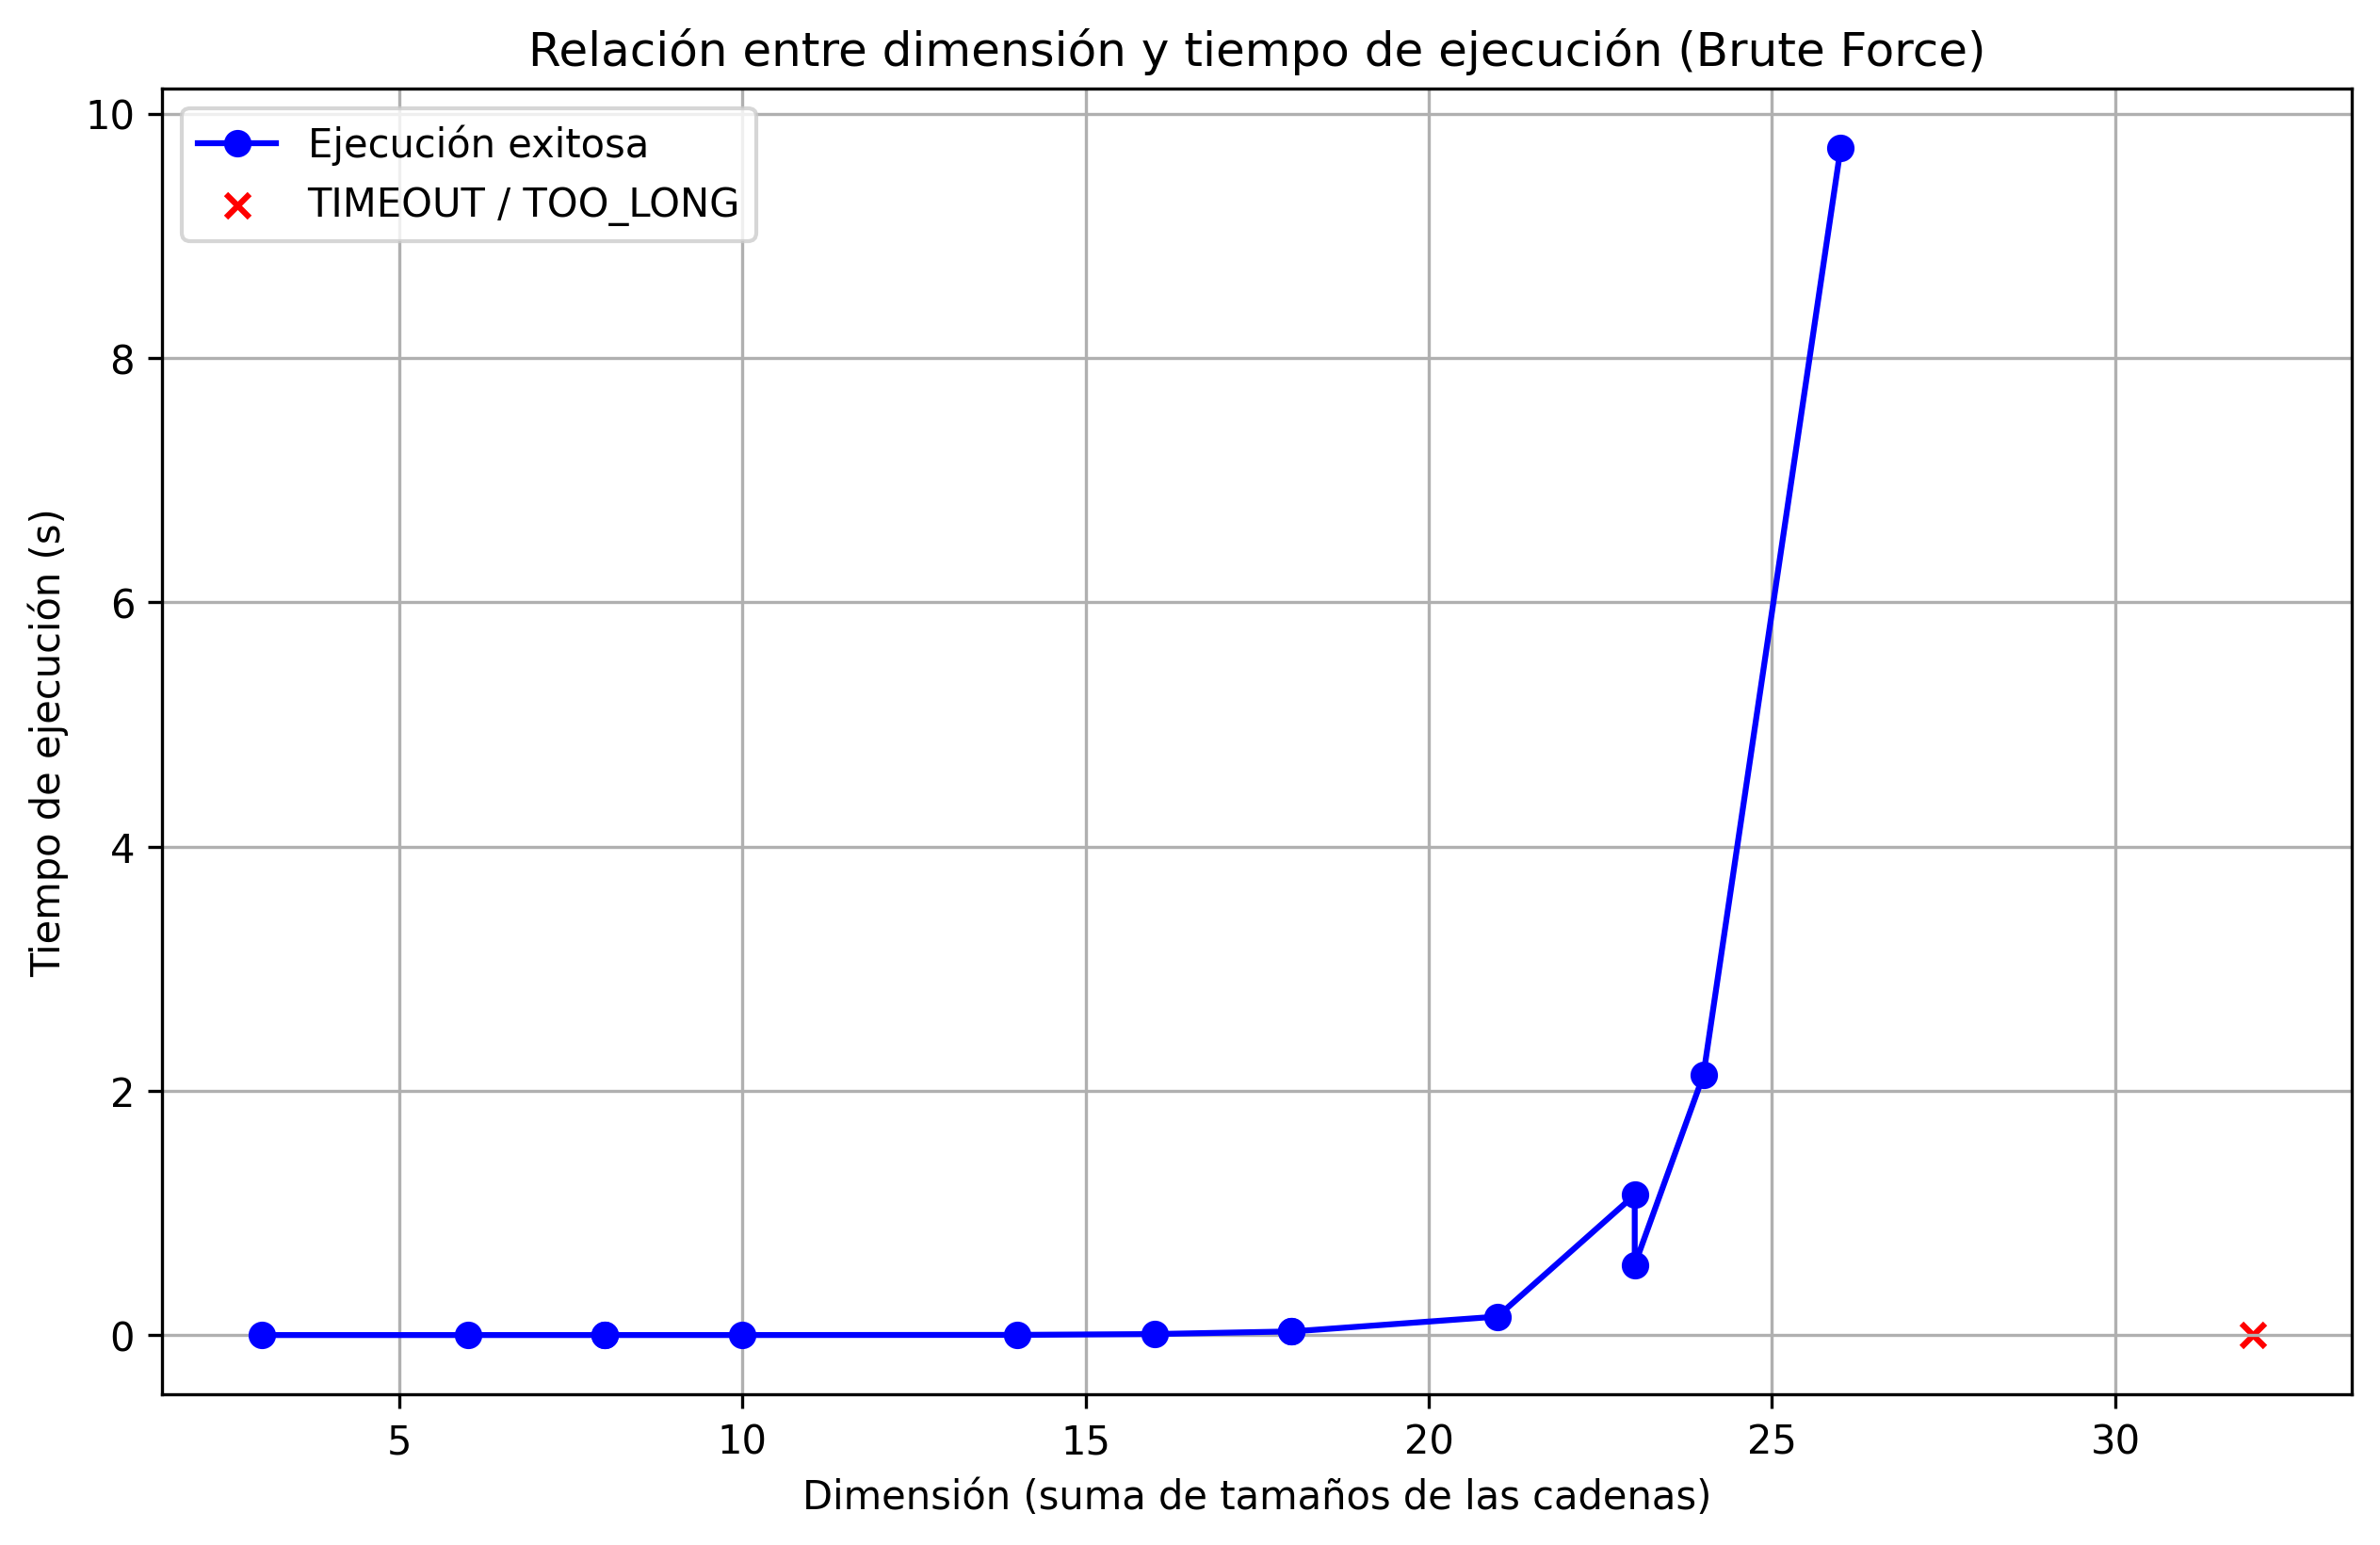
\includegraphics[width=0.7\linewidth]{report/images/dtfb.png}
    \caption{Tiempo de ejecución del algoritmo de Fuerza Bruta.}
\end{figure}
\begin{figure}[h]
    \centering
    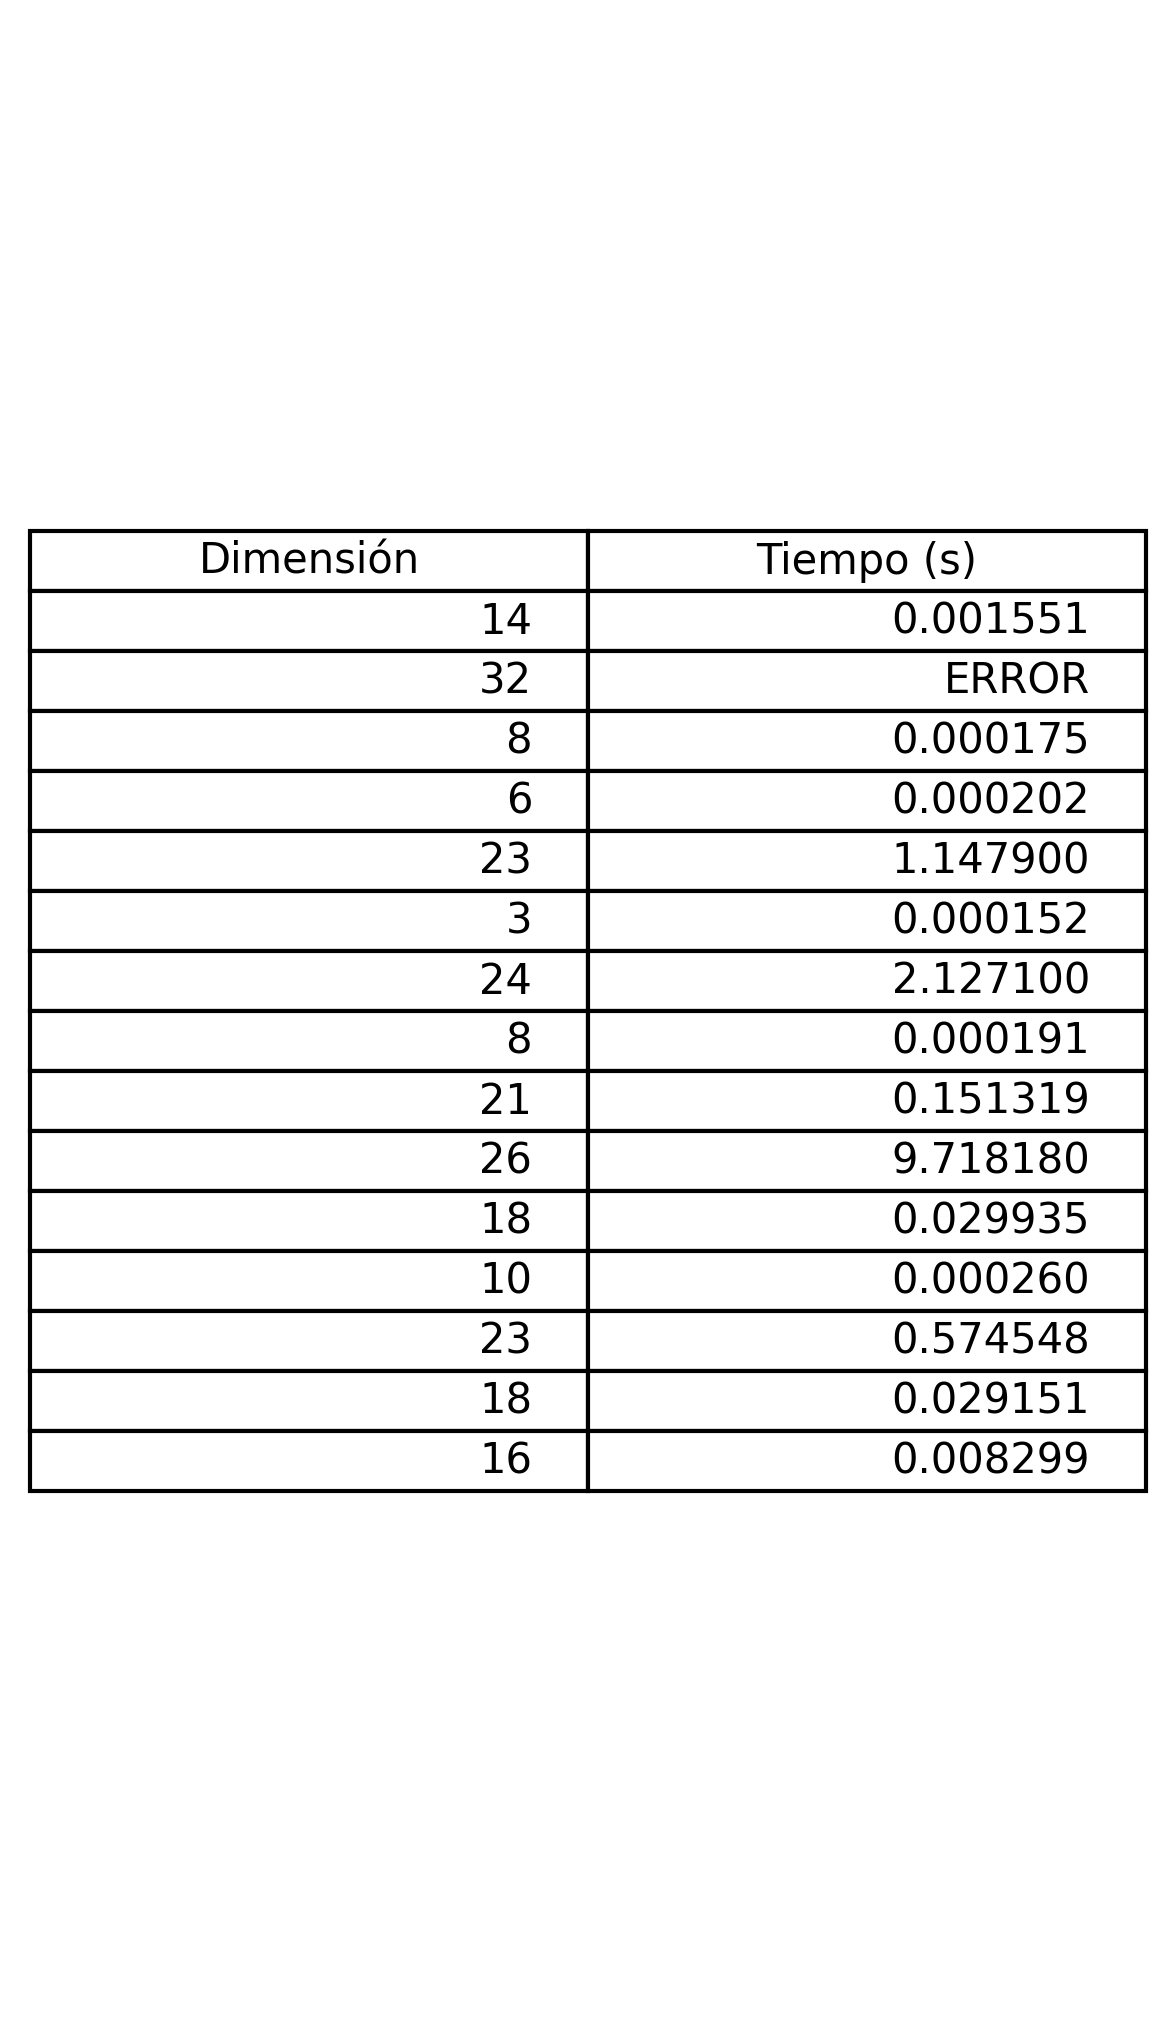
\includegraphics[width=0.7\linewidth]{report/images/dtfbt.png}
    \caption{Tiempo de ejecución del algoritmo de Fuerza Bruta.}
\end{figure}

\begin{figure}[h]
    \centering
    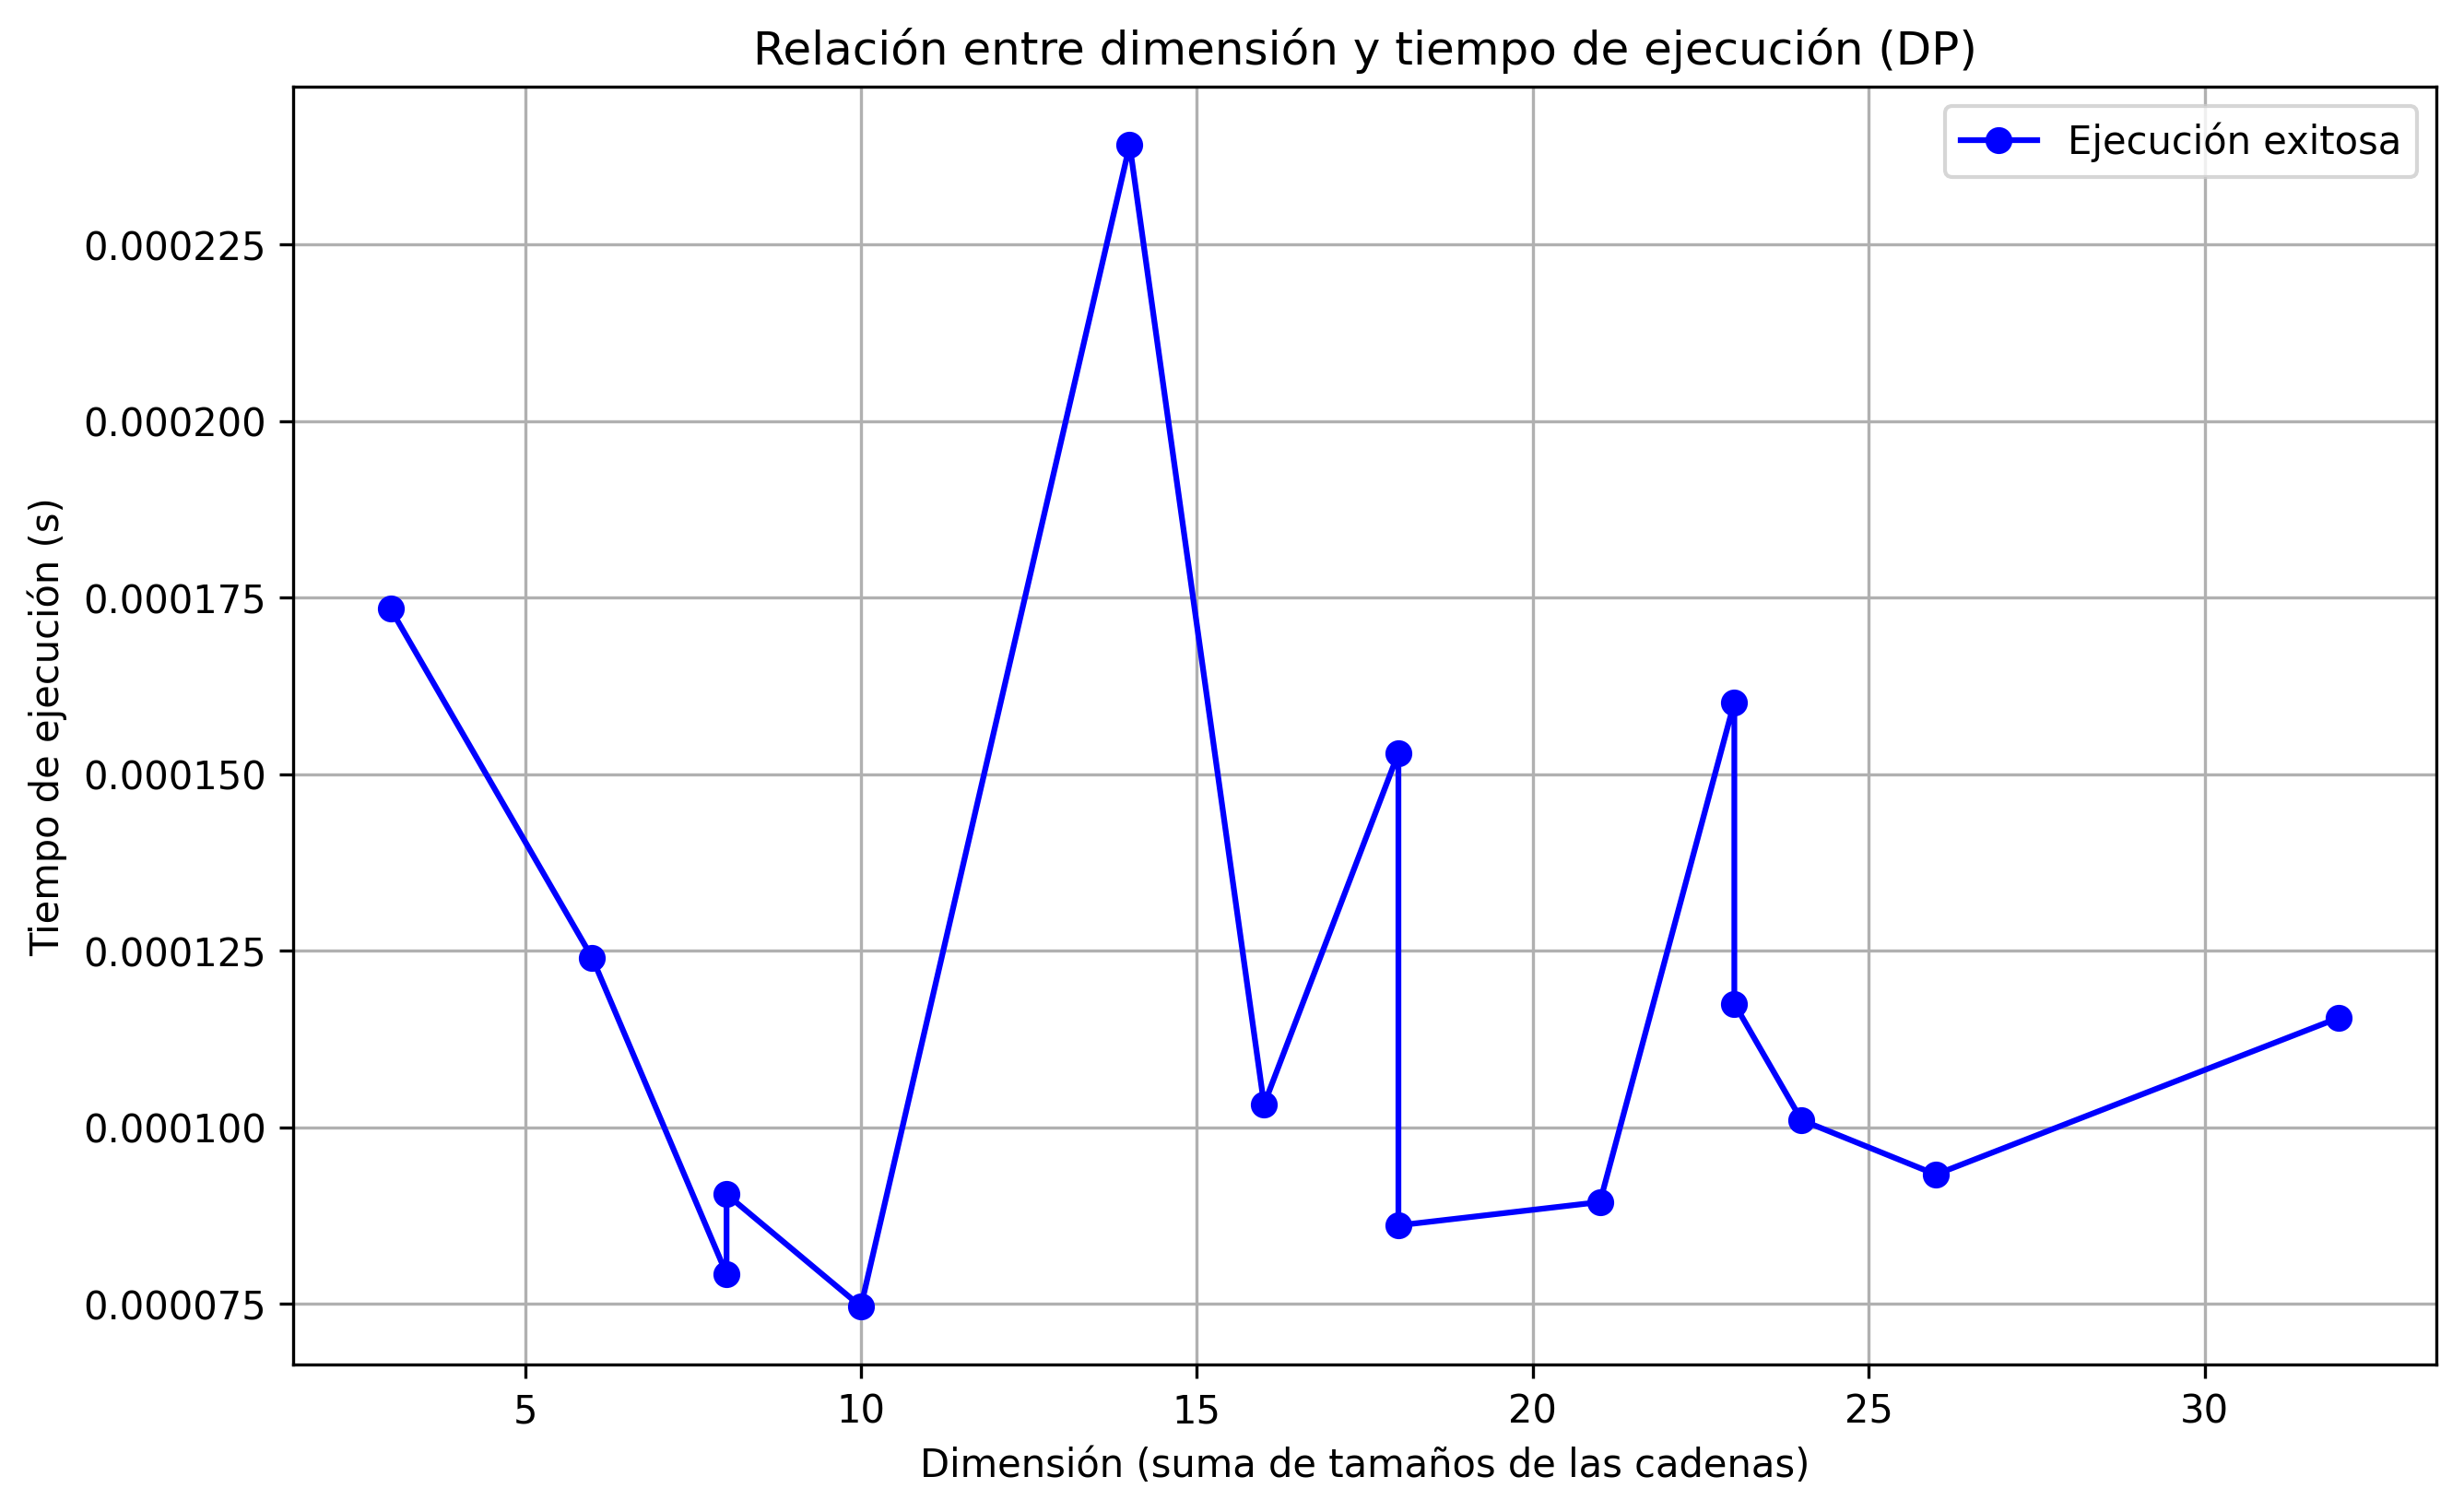
\includegraphics[width=0.7\linewidth]{report/images/dtdp.png}
    \caption{Tiempo de ejecución del algoritmo de Programación Dinámica.}
\end{figure}
\begin{figure}[h]
    \centering
    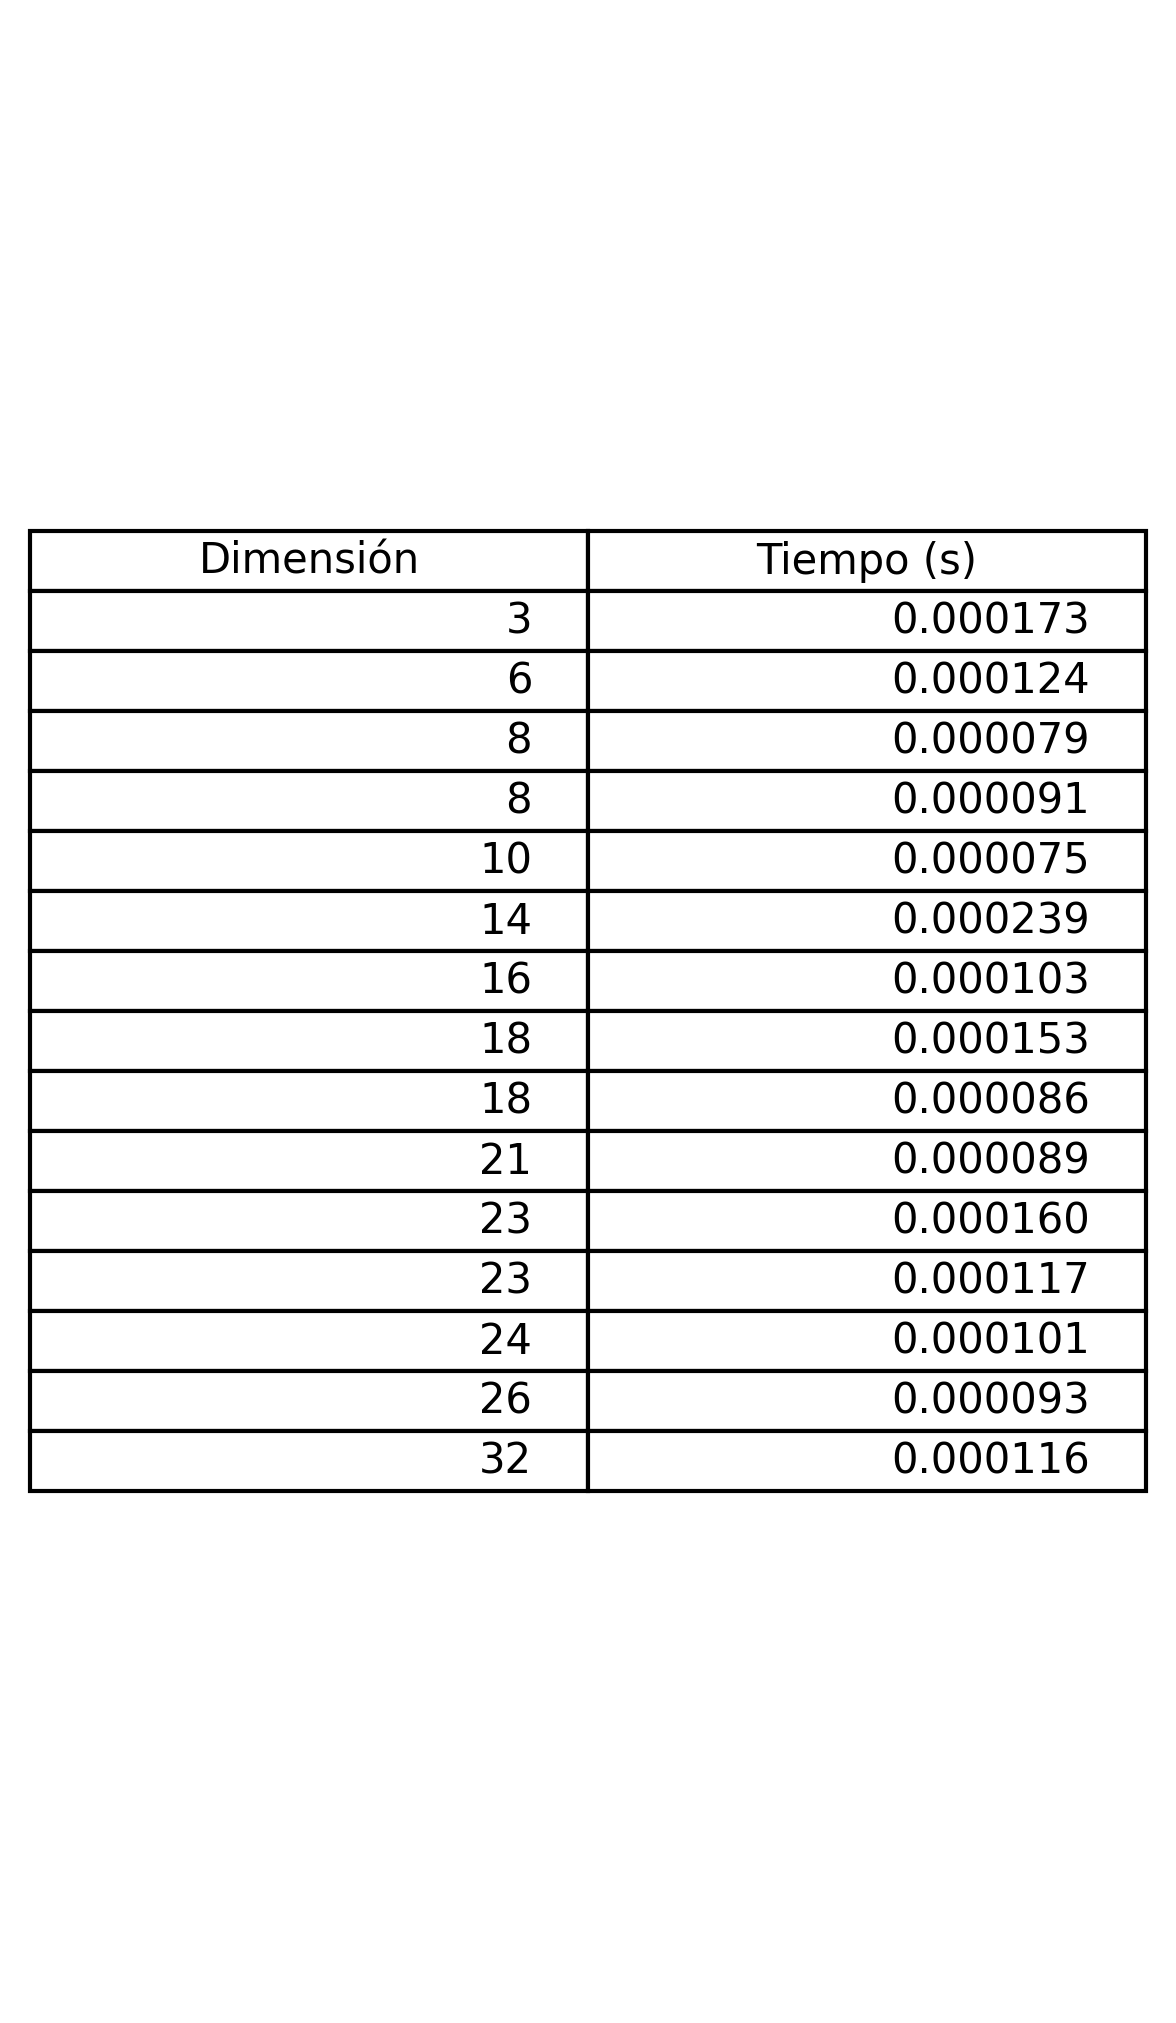
\includegraphics[width=0.7\linewidth]{report/images/dtdpt.png}
    \caption{Tiempo de ejecución del algoritmo de Programación Dinámica.}
\end{figure}

Los datos analizados provienen de los archivos que se generan en  \texttt{data/measurements/*.txt} al ejecutar cada enfoque con el input.

4.3. Análisis Comparativo

Los resultados obtenidos reflejan las grandes diferencias en complejidad entre ambos enfoques:

    Fuerza Bruta muestra un crecimiento exponencial en tiempo de ejecución, 
    alcanzando el límite de 5 minutos en entradas de 23 elementos en adelante Por ejemplo, para entradas de longitud 26, el tiempo supera los 9 segundos, y para 32 se marca como “ERROR” por exceder el tiempo permitido. Esto concuerda con su complejidad exponencial teórica $O(2^{n + m})$.


    Programación Dinámica, en comparacion mantiene un tiempo de ejecución muy bajo 
    incluso para cadenas de un mayor tamaño como 32,lo que reafirma su eficiencia $O(n \cdot m)$. La estabilidad de los tiempos 
    indica que este enfoque es más escalable y adecuado para aplicaciones con datos más 
    extensos.

Esta diferencia valida la eleccion de programación dinámica como la solución mas favorable para el contexto en que se analizo, mientras que la fuerza bruta puede ser útil solo para 
instancias muy pequeñas o como referencia conceptual.